\documentclass[11pt,twocolumn]{article} 
\usepackage{geometry}
 \geometry{
  a4paper,
  left=17.5mm,
  right=17.5mm,
  bottom=15mm,
  top=15mm
 }
\usepackage[english]{babel}
\usepackage{tikz}
\usetikzlibrary{decorations.pathreplacing}
\usepackage{textcomp}
\usepackage{float}
\usepackage{amsmath}
\tikzset{XOR/.style={draw,circle,append after command={
        [shorten >=\pgflinewidth, shorten <=\pgflinewidth,]
        (\tikzlastnode.north) edge (\tikzlastnode.south)
        (\tikzlastnode.east) edge (\tikzlastnode.west)
        }
    }
}
\usepackage{graphicx,booktabs,array}

\title{\bf \Huge A practical application of EOS\textregistered{} projection geometry}
\author{{\bf \Large Anthony J. Lombard$^{1,2}$}\\
  $^1$ Medical Computing Team, Kitware Inc.,\\
  Albany, NY, USA\\
  $^2$ Department of Computer Science, Clarkson University,\\ 
  Potsdam, NY, USA
  }
\date{April 26th 2024}

\begin{document}
\maketitle

he report should contain an abstract within 300 words. The report should have a self-contained, citation-free abstract and state briefly the purpose of the research, methodology, key results and major conclusions. Abstract should be in a single paragraph with running sentences. Do not use any subheading or point list within the abstract. Also, non-standard or uncommon abbreviations should be avoided, but if essential they must be defined at their first mention in the abstract itself.  
\noindent
{\bf Keywords:} Authors are advised to write 3-5 keywords related to the project, separated by comma. 

\section{Introduction}

The EOS\textregistered{} radiographic scanner is unique system that allows for full-body radiography. 
The ability to be able to quickly render Digitally Reconstructed Radiographs (DRRs) is a necessary step to perform
many different forms of analysis later on, such as 2D-3D registration. 

While previous publications have defined volume-order rendering techniques for this scanner \cite{groisser2019geometry},
there has not been any development towards image-order rendering. Image-order techniques have a few advantages over 
volume-order techniques. Mainly, it is easier to parallelize image-order techniques for faster computation. It is also 
easier to render regions of interest (ROI) rather than the entire image.

This paper provides a detailed overview of DRR rendering using ray-casting, an overview of the EOS\textregistered{} 
geometry, the modified ray-casting approach used to simulate the EOS\textregistered{} scanner, and a comparison 
between radiographs captures on an EOS\textregistered{} scanner and simulated DRRs. 

\section{Ray-casting / DRR generation}
The basic idea of ray-casting is sending rays from a point source through a 3D scene to determine the value at each 
pixel in the final image. 

Let our camera be a static point in world space, C. 
Let the current pixel in the image be some point on the image plane in world space, I. 
Then the direction of travel for our ray would be the normalized result of I-C, we will call this R.

We can express a point, P, along this ray using the parametric form. Where t is the distance traveled along the ray.
\begin{equation}
  P = C + t * R
\end{equation}


\begin{equation}
  \text{pixel intensity} = \sum_{t=0,step\_size}^{dist(I,C)} value(C+t*R)
\end{equation}

In a naive approach, we could now get the intensity of each pixel using equation (2).
Where the function $dist$ returns the distance between two points, in this case the camera, C, and the pixel position I.
And the function $value$ returns the value of the volume at a given point, if the point lies outside of the volume it 
returns 0.
The $step\_size$ is the amount that t increments each iteration of the summation.

However, this approach has two major problems. 
First, it is likely that the volume does not take up the entire space between 
points C and I, so there would be many needless steps along the ray. We can solve this by using ray box intersection
to determine the values of t, if any, that the volumes resides in. Second, since the voxels of the volume are not 
clustered directly next to each other, there is some physical distance between points within the volume, it is likely 
that the point P won't fall directly on the center of a voxel. In the naive approach, we could simply take the value 
from the closest voxel. A better approach is to take the weighted average of the eight closest voxels, this is 
trilinear-interpolation \cite{Yoder_2003}.

\subsection{Ray box intersection}
In order to reduce the number of iterations needed to traverse each ray, ray-box intersection was utilized to 
determine the values for t that the volume fits between. We define the box based on the position and size of the volume
for all three axes. In total six planes are computed, in general this can be represented by the near and far planes
for each axis.
\begin{equation}
  box_{near} = \{X_{near}, Y_{near}, Z_{near}\}
\end{equation}
\begin{equation}
  box_{far} = \{X_{far}, Y_{far}, Z_{far}\}
\end{equation}
For each axis, the minimum and maximum extents for the box had the corresponding axial component 
of the ray origin subtracted from the extent, then the result of the subtraction is divided by the axial component 
of the ray direction. For example using the X-axis.
\begin{gather*}
  t_{xn} = (X_{near} - ray\_origin.x) / ray\_direction.x\\
  t_{xf} = (X_{far} - ray\_origin.x) / ray\_direction.x
\end{gather*}

We then find the minimum and maximum values for each axis and organize the results into two arrays, $tMin$ and $tMax$.
Where $tMin.x = min(t_{xn},t_{xf})$. Then the value for the near plane s computed as the maximum of the
$tMin$ array. Likewise the value for the far plane is computed as the minimum of the $tMax$ array.

If the value of the near plane is greater than that of the far plane, the ray missed the box. In which case we can end
computation early, saving more time and resources. 
\cite{glassnerIntro}

\section{Overview of the EOS\textregistered{} geometry}

The EOS\textregistered{} radiographic scanner contains two X-ray sources, that are mounted orthgonally from one
another. The two sources are physically linked so the two radiographic images are collected in unison. During a 
scan the sources are moved vertically.

\begin{figure}[H]
  \centering
  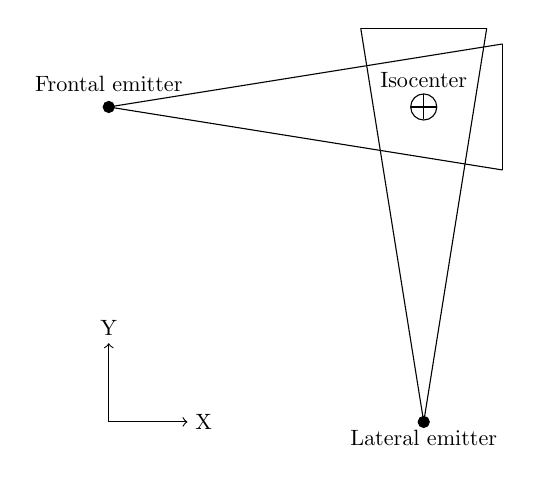
\begin{tikzpicture}
    % Frontal emitter
    \draw (0,0) -- (5,.8);
    \draw (0,0) -- (5,-.8);
    \draw (5,.8) -- (5,-.8);
    \filldraw (0,0) circle (2pt) node[above,scale=0.8] at (0,0.1) {Frontal emitter};

    % Lateral emitter
    \draw (4,-4) -- (3.2,1);
    \draw (4,-4) -- (4.8,1);
    \draw (3.2,1) -- (4.8,1);
    \filldraw (4,-4) circle (2pt) node[below, scale=0.8] {Lateral emitter};

    % Isocenter
    \draw (4,0) node[XOR]{} node[above,scale=0.8] at (4, 0.15) {Isocenter};

    % Axis
    \draw[->] (0,-4) -- (0,-3) node[above,scale=0.8] {Y};
    \draw[->] (0,-4) -- (1,-4) node[right,scale=0.8] {X};
  \end{tikzpicture}

  \caption{Top-down view of the EOS\textregistered{} geometry}
\end{figure}

Each source is at a known fixed position relative to each sources respective detector and the isocenter. 

\begin{figure}[H]
  \centering
  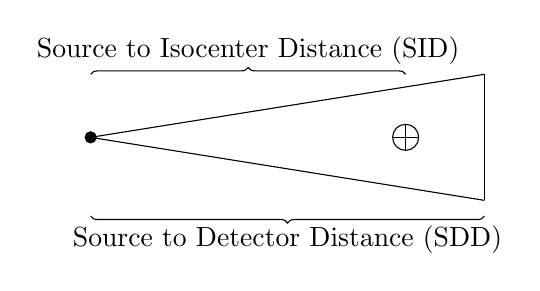
\begin{tikzpicture}
    \path[draw,decorate,decoration={brace}] (0,.8) -- (4,.8) node[midway,above]{Source to Isocenter Distance (SID)};
    % Frontal emitter
    \draw (0,0) -- (5,.8);
    \draw (0,0) -- (5,-.8);
    \draw (5,.8) -- (5,-.8);
    \filldraw (0,0) circle (2pt) node[above,scale=0.8] at (0,0.1) {};

    % Isocenter
    \draw (4,0) node[XOR]{} node[above,scale=0.8] at (4, 0.15) {};

    \path[draw,decorate,decoration={brace,mirror}] (0,-1) -- (5,-1) node[midway,below]{Source to Detector Distance (SDD)};
  \end{tikzpicture}
  \caption{Known fixed distances}
\end{figure}

Each radiograph image collected by the system can be of arbitrary size defined by the number of rows, R,
and the number of columns, C. The spacing between pixel centers is also known, the horizontal spacing is defined as
$\lambda$ and the vertical spacing is defined as $\lambda_z$.

\begin{figure}[H]
  \centering
  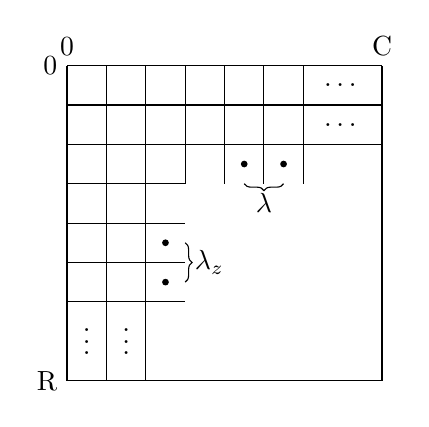
\begin{tikzpicture}[scale=2]
    \draw (0,0) node[above]{0} -- (2,0) node[above]{C};
    \draw (0,0) node[left] {0} -- (0,-2) node[left] {R};
    \draw (0,-2) -- (2,-2);
    \draw (2,-2) -- (2,0);

    % Horizontal Lines
    \draw (0,-0.25) -- (2,-.25);
    \draw (0,-0.5) -- (2,-.5);
    \draw (0,-0.75) -- (.75,-.75);
    \draw (0,-1) -- (.75,-1);
    \filldraw (0.625,-1.125) circle (0.5pt);
    \draw (0,-1.25) -- (.75,-1.25);
    \filldraw (0.625,-1.375) circle (0.5pt);
    \draw (0,-1.5) -- (.75,-1.5);

    \node[] at (1.75,-.125) {\dots};
    \node[] at (1.75,-.375) {\dots};
    
    \path[draw,decorate,decoration={brace}] (0.75 ,-1.125) -- (0.75,-1.375) node[midway,right]{$\lambda_z$};

    % Vertical Lines
    \draw (.25,0) -- (.25,-2);
    \draw (.5,0) -- (.5,-2);
    \draw (.75,0) -- (.75,-.75);
    \draw (1,0) -- (1,-.75);
    \filldraw (1.125,-.625) circle (0.5pt);
    \draw (1.25,0) -- (1.25,-.75);
    \filldraw (1.375,-.625) circle (0.5pt);
    \draw (1.5,0) -- (1.5,-.75);

    \node[] at (.125,-1.70) {\vdots};
    \node[] at (.375,-1.70) {\vdots};

    \path[draw,decorate,decoration={brace,mirror}] (1.125 ,-0.75) -- (1.375,-0.75) node[midway,below]{$\lambda$};
  \end{tikzpicture}
  \caption{Radiograph size and spacing}
\end{figure}


\section{EOS\textregistered{} geometry for DRR generation}

Note the subscript $f$ denotes a parameter specific to the frontal source. 
Likewise the subscript $l$ denotes a parameter specific to the lateral source.

Let v be the current vertical index in the DRR, where $v \in [0,R)$.

Let u be the current horizontal index in the DRR, where $u \in [0,C)$.

Let $z_0$ be the initial height of the scanner, then the current height of the scanner can then be defined as the 
current vertical index scaled by the vertical pixel spacing, then offset from the initial scanner height.

\begin{equation}
  z = z_0 - \lambda_z * v
\end{equation}

Defining the isocenter to be the point (0, 0, z) we can get the following positions, in world space, for the frontal 
and lateral sources.

\begin{equation}
  s_f = \{-sid_f,0,z\}
\end{equation}

\begin{equation}
  s_l = \{0,-sid_l,z\}
\end{equation}

The distance between the isocenter and each detector can be defined as the difference between each sources sdd and sid.
The position along each detector can be defined as the current horizontal index off set by half of the total number 
of columns in the image. This value then gets scaled by the horizontal pixel spacing and then divided by the focal
length. The ratio of sid to sdd is used as the focal length.

Therefore the current position on the detector, in world space, can be defined by the following equations.
\begin{equation}
  d_f = \{sdd_f-sid_f, \frac{(u - \frac{C_f}{2}) \cdot \lambda_f \cdot sdd_f}{sid_f},z\}
\end{equation}

\begin{equation}
  d_l = \{\frac{(u - \frac{C_l}{2}) \cdot \lambda_l \cdot sdd_l}{sid_l}, sdd_l-sid_l, z\}
\end{equation}

The ray-casting algorithm described in section 2, was then modified so the camera position was defined by $s$. The ray direction was then defined as the normalized result of $d-s$ the rest of the
algorithm was left as is.

\section{Results}

\section{Assessment of results}
\subsection{Finding the similarity between images}


\section{Conclusions}

\section{Future work}

\section{Acknowledgments}

* Amy
* Sean and Natasha
* Trey
* Bea
* JC

\bibliographystyle{plain}

\bibliography{manuscript_references}

\end{document}
